\clearpage

\begin{usecase}
    \addheading{Use-Case Description}
    \addsingletwocolumnrow{Name}{ugManageCrisis}
    \addsingletwocolumnrow{Scope}{System}
    \addsingletwocolumnrow{Altitude}{Summary}
    \addrowheading{Parameters}
    \addnumberedsinglerow{}{none}
    \addrowheading{Primary actor(s)}
    \addnumberedsinglerow{}{\msrcode{\msrcode{actCoordinator[active]}}}
    \addrowheading{Secondary actor(s)}
    \addnumberedsinglerow{}{none.}
    \addrowheading{Goal(s) description}
    \addsinglerow{The goal is to use all operations available to the coordinator for the successful handling of a crisis or an alert received by our system.}
    \addrowheading{Reuse}
    \addnumberedsinglerow{}{\msrucname{oeSetCrisisStatus}}
    \addnumberedsinglerow{}{\msrucname{oeSetCrisisHandler}}
    \addnumberedsinglerow{}{\mrsucname{oeRequestEMSAssistance}}
    \addnumberedsinglerow{}{\msrucname{oeReportOnCrisis}}
    \addnumberedsinglerow{}{\msrucname{oeCloseCrisis}}
    \addrowheading{Protocol condition(s)}
    \addnumberedsinglerow{}{the \msricrash system has been started}
    \addnumberedsinglerow{}{the \msrcode{actCoordinator} has been added to the system.}
    \addnumberedsinglerow{}{the \msrcode{actCoordinator} has safely logged on to the system.}
    \addnumberedsinglerow{}{the \msrcode{actDomainExpert} has validated the alert.}
    \addnumberedsinglerow{}{the \msrcode{actCoordinator} has the right domains of expertise to manage this alert.}
    \addrowheading{Pre-condition(s)}
    \addnumberedsinglerow{}{none}
    \addrowheading{Main post-condition(s)}
    \addnumberedsinglerow{}{there is a crisis whose related information has been changed.}
    \addrowheading{Main success steps}
    \addalphanumberedsinglerow{}{the actor \msrcode{actCoordinator} executes the  \msrucname{oeSetCrisisHandler} use case.}
    \addalphanumberedsinglerow{}{the actor \msrcode{actCoordinator} executes the \msrucname{oeSetCrisisStatus} use case.}
    \addalphanumberedsinglerow{}{the actor \msrcode{actCoordinator} executes the \msrucname{oeReportOnCrisis} use case.}
    \addalphanumberedsinglerow{}{the actor \msrcode{actCoordinator} executes the \msrucname{oeCloseCrisis} use case.}
    \addrowheading{Step Constraints Ordering and Extensions}
    \addnumberedsinglerow{}{Step a) must be executed first.}
    \addnumberedsinglerow{}{Step d) must be executed last.}
    \addnumberedsinglerow{}{Steps b)to c) can be executed multiple times in order to manage a crisis.}
\end{usecase}

\clearpage

\begin{figure}[htbp]
\begin{center}
\scalebox{0.95}{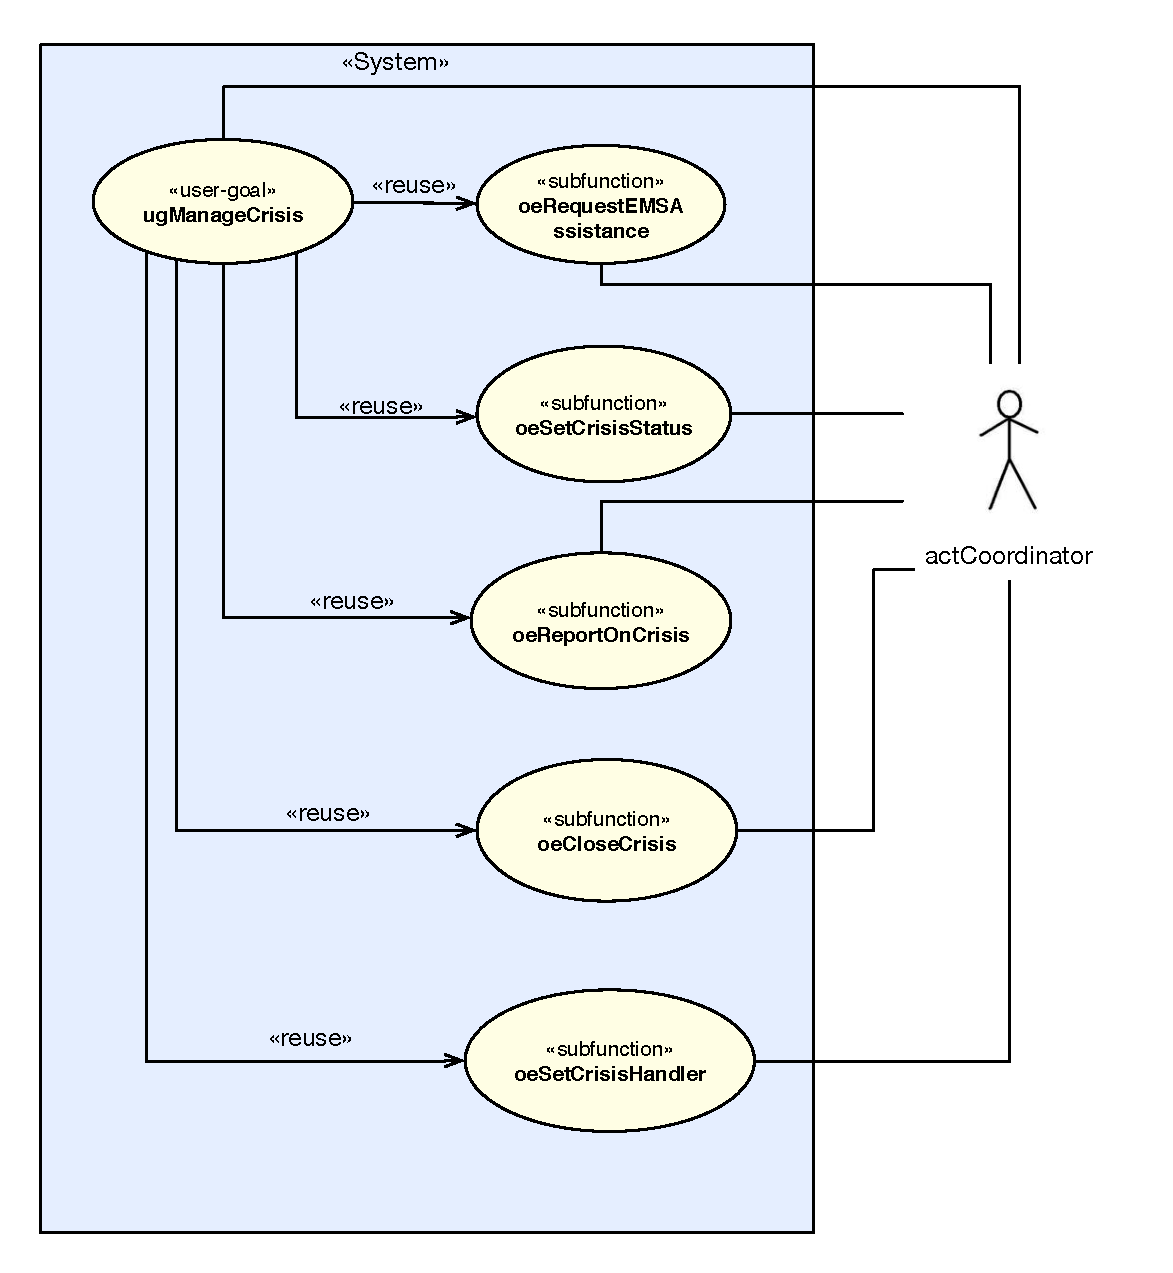
\includegraphics[width=180mm]{./images/UgManageCrisis.eps}\normalsize}
\end{center}
\caption[\msricrash Use Case Diagram: UgManageCrisis Diagram]{\msricrash Use Case Diagram: UgManageCrisis}
\label{fig:icrash-RE-UCD-UgManageCrisis}
\end{figure}
\vspace{0.5cm}

